% !TEX root = ../Sesiones-TDA-Ejercicios.tex

%%%%%%%%%%%%%%%%%%%%%%%%%%%%%%%%%%%%%%%%%%%%%%%%%%%%%%%%%%%%%%%%%%%%%%%%%%%%%%%%%%%%
%%%%%%%%%%%%%%%%%%%%%%%%%%%%%%%%%%%%%%%%%%%%%%%%%%%%%%%%%%%%%%%%%%%%%%%%%%%%%%%%%%%%

\


\centerline{\Large \bf Python}


%%%%%%%%%%%%%%%%%%%%%%%%%%%%%%%%%%
%%%%%%%%%%%%%%%%%%%%%%%%%%%%%%%%%%
% --------------------------------------------------------
\section*{2.E Python}
\addcontentsline{toc}{section}{2.E Python}


Para la implementación de los TDAs se usará Python. En esta sección vamos a dar un repaso breve, pero lo suficientemente completo de este lenguaje como para abordar los ejercicios de esta sesión.


%%%%%%%%%%%%%%%%%%%%%%%%%%%%%%%%%%
%%%%%%%%%%%%%%%%%%%%%%%%%%%%%%%%%%
% --------------------------------------------------------
\subsection*{2.E.1 Breve Historia de Python}
\addcontentsline{toc}{subsection}{2.E.1 Breve Historia de Python}





\key[red]{Python} es un lenguaje creado por Guido van Rossum (Haarlem, Países Bajos, 31/1/1956).
 En diciembre de \key{1989}  buscó un proyecto de programación como hobby para pasar las vacaciones de Navidad basado en el lenguaje \textbf{ABC} (script).
 Eligió el nombre de Python para el proyecto (como fan de Monty Python's Flying Circus)

En \key{1991} van Rossum publicó el código 0.9.0 por 1$^{\underline{a}}$ vez en \cm[blue]{alt.sources}. Tiene un ruerte influencia de \textbf{Modula} y  presenta clases con \cm{herencia}, manejo de \cm{excepciones}, funciones y tipos modulares. Se basa en sistema de \cm{módulos}.
La primera versión de Python se lanzó con licencia de Código Abierto. \url{https://docs.python.org/3/license.html}
 
En \key{1994} se formó \cm[blue]{comp.lang.python}, el foro de discusión principal de Python. En \key{1999} se lanza la primera versión de la serie 1.0 donde se introduce programación funcional así como las funciones \cm{reduce()}, \cm{filter()} y \cm{map()} inspiradas en \textbf{Lisp}.
En \key{1999} van Rossum realizó una propuesta a DARPA (Agencia de Proyectos de Investigación Avanzados de Defensa) llamada \cm[black!80!blue]{Computer Programming for Everybody}, consiguiendo que el lenguaje fuera patrocinado.

En mayo de \key{2000}, Guido y el equipo central de desarrollo de Python formaron  \cm[black]{BeOpen PythonLabs} de BeOpen.com. Sacan la versión 2.0.
En octubre de 2000, el equipo de \cm[black]{PythonLabs} se trasladó a Digital Creations (ahora Zope Corporation; consulte https://www.zope.org/). 
En \key{2001}, se formó \href{https://www.python.org/psf/}{Python Software Foundation}, una organización sin fines de lucro creada específicamente para poseer propiedad intelectual relacionada con Python. 

Desde la versión 2.1. todas tienen  la \textit{Python Software Foundation License}.

\begin{itemize}

\item \key{Python 2.x:} generación de listas basada en la programación funcional \textbf{Haskell}, recolección de basura (inventado por John McCarthy como parte de \textbf{Lisp}),  generadores (basado en Icon), la unificación de tipo en Python (escritos en \textbf{C}) y clases (escritos en Python) dentro de una jerarquía (lo convierte en un lenguaje basado en un modelo POO puro). La v.2.7 dejó de tener soporte el 1/1/2020.

\item \key{Python  3.x} (desde 2008): Hace limpieza de código y deja de ser complatible con 2.x.. Incluye una lista interminable de mejoras en cada versión. La última en la  \href{https://docs.python.org/es/3.10/whatsnew/3.10.html}{ver. 2.10.2} del 21/2/2022 que incluye la \cm[black]{coincidencia de patrones estructurales}.
\end{itemize}




%%%%%%%%%%%%%%%%%%%%%%%%%%%%%%%%%%
%%%%%%%%%%%%%%%%%%%%%%%%%%%%%%%%%%
% --------------------------------------------------------
\section*{2.E.2 Características y Uso}
\addcontentsline{toc}{subsection}{2.E.2 Características y Uso}


El \href{https://www.tiobe.com/tiobe-index/programming-languages-definition/}{índice TIOBE} calcula la popularidad de los lenguajes de programación usando 25 motores de búsqueda de distintos países (google, wikipedia, amazon). La popularidad se asocia al uso:
{Mayor uso \textrightarrow más dudas \textrightarrow más búsquedas}

En octubre de 2021 Python ocupó el primer puesto en el \href{https://www.tiobe.com/tiobe-index/}{índice Tiobe}, convirtiéndose en el tercer lenguaje que lidera el índice en sus más de 20 años de existencia. Python, C y Java acaparan el 42\% de "la popularidad" de todos los lenguajes de programación.



\noindent Inicialmente los \textbf{objetivos} marcados por Guido cuando lo presentó a DARPA:
\begin{itemize}
\item Python debería ser \key{fácil}, intuitivo y tan potente como sus principales competidores.
\item El proyecto sería de \key{código abierto} para que cualquiera pudiera colaborar.
\item El código escrito en Python sería tan comprensible como cualquier texto en \key{inglés}.
\item Python debería ser apto \key{para las actividades diarias} permitiendo la construcción de prototipos en \textbf{poco tiempo}.
\end{itemize}

\noindent Lo que es hoy en día:

\begin{itemize}
\item \key{Multiplataforma} (Windows, Linux/UNIX, macOS,  iOS, iPadOS y otros).
\item Lenguaje de programación \key{interpretado}.
\item \key{Multiparadigma:} imperativo (modular y orientado a objetos) y funcional.
\item \key{Dinámico:} {\small 1) No necesita declaración explícita del tipo, 
$ $\phantom{Dinámico: }  2) Se determina en tiempo de ejecución.}
\item \key{Fuertemente tipado} (no se puede cambiar el tipo de dato). 
No se puede hacer \cm{'1'+2}.
\item Permite la \key{inclusión} de módulos en C, C++.
De hecho está implementado sobre C.
\end{itemize}




\noindent 
 Su gran popularidad se debe, en parte, a que hoy en día es \textbf{EL} lenguaje de programación de referencia para 

\begin{itemize}
\item El \key{desarrollo web.}
\begin{itemize}
\item Pyramid, Django y Flask.
\item Frameworks que integran protocolos y reducen el tiempo de desarrollo.
\end{itemize}

\item \key{Ciencias de los datos}
\begin{itemize}
\item NumPy (matrices), Pandas (manipulación y limpieza), Plotly y Seaborn (visualización estadística de datos), Shap (explicación de modelos), etc. 
\item Bibliotecas de desarrollo ayudan a extraer información  de los datos
\end{itemize}

\item \key{Inteligencia Artificial y Aprendizaje Automático}
\begin{itemize}
\item Keras / Tensorflow / Scikit-learn / PyTorch (machine learning), OpenCV (visión artificial), PyKE (programación lógica), ...
\end{itemize}

\item \key{Aplicaciones empresariales}
\begin{itemize}
\item Es un lenguaje robusto que puede manejar múltiples \textbf{solicitudes} de \textbf{bases de datos} a la vez.
\item Legibilidad, funcionalidad y escalabilidad permanece igual.
\end{itemize}
\end{itemize}


\noindent También se usa en otros ámbitos como los siguientes:

\begin{itemize}

\item \key{Sector educativo}
\begin{itemize}
\item  Fácil de aprender para principiantes ya que su sintaxis ``coincide'' con la del inglés.
\item Potenciado por el desarrollo de cursos y programas educativos on-line.
 \textit{Python} tiene 123 resultados en EdX y 878 resultados en Coursera.
\end{itemize}

\item \key{Web scraping}
\begin{itemize}
\item Recopila información de las páginas web.
\item Ejemplos son PythonRequest, Selenium, MechanicalSoup.
\end{itemize}

\item \key{Desarrollo de Juegos}
\begin{itemize}
\item Pygame, PyKyra, Pyglet, PyOpenGL, Kivy, Panda3D, Cocos2D, ...
\item No es lo más usado, pero a veces surgen juegos destacados. P.e. Campo de batalla 2 (2000)
\end{itemize}


\item\key{ Desarrollo de software}
\begin{itemize}
\item Simplica el proceso de desarrollo de software para aplicaciones complejas.
\item Se usa para la gestión del proyecto, como lenguaje de apoyo.
\end{itemize}

\item \key{GUI de escritorio}
\begin{itemize}
\item Tkinter, PyQt, PyGUI y WxPython
\item Crear GUI de alta calidad de manera eficiente.
\end{itemize}

\item \key{Sistemas operativos}
\begin{itemize}
\item Scripts para mantenimiento del sistema.
\item macOS no puede vivir sin Python 2.7 ... hasta la ver. 12.3 (Monterey), pero incluye la versión 3 con XCode.
\end{itemize}
\end{itemize}


Algunas aplicaciones conocidas que usan Python son:


\begin{itemize}
\item Windows (la instalación asistida)
\item Bit Torrent (descargas p2p)
\item Google App Engine (servicio de alojamiento web)
\item Ubuntu Software Center (gestor de aplicaciones)
\item Dropbox (servicio de almacenamiento)
\item Uber (lo usa con Big Data Analytics de IBM)
\item Blender (Modelado 3D)
\item Instagram (red social)
\item Pinterest (red social)
\item Reddit (red social)
\item Youtube (red social)
\item Spotify (servicio de streaming de música)
\item Netflix (servicio de streaming de video)
\end{itemize}




%%%%%%%%%%%%%%%%%%%%%%%%%%%%%%%%%%
%%%%%%%%%%%%%%%%%%%%%%%%%%%%%%%%%%
% --------------------------------------------------------
\subsection*{2.E.3 Variables, Expresiones y Conversión de Tipo}
\addcontentsline{toc}{subsection}{2.E.3 Variables, Expresiones y Conversión de Tipo}



\paragraph{Tipos de Datos.}
En programación imperativa se distinguen dos tipos de datos: elementales y compuestos.

\begin{itemize}

\item \textbf{Tipos de datos primitivos (o elementales)}

\begin{itemize}
\item Formado por un único elemento.
\item Tipos: carácter,  númerico,  booleano,  enumerado.
\end{itemize}


\item \textbf{Tipos de datos compuestos}

\begin{itemize}
\item   Formado por una agrupación de elementos.
\item Tipos: string, array,  registro,  conjunto,  lista, diccionario.
\end{itemize}

\end{itemize}


\paragraph{Variable y expresiones.}
Las \concepto{variables} son las ubicaciones de almacenamiento de los datos. 
Cada variable se caracteriza por su \textbf{nombre} y el \textbf{valor} almacenado.
\key{Declarar} una variable es dar la orden para establecer el tipo de dato que se almacenará  e identificar la zona de memoria con el identificador establecido.
\key{Asignar} valor a una variable es almacenar una información en la zona de memoria del identificador. La asignación se realiza con \cm{=}.
La primera asignación se llama \key{inicialización}.
Una \concepto{constante} es una variable para la que solo se puede realizar la inicialización (no caben más asignaciones).


\cm[red]{Python} es dinámicamente tipado:
	\begin{itemize}
	\item No existe la declaración de forma explícita.
	\item Al realizar una asignación, de forma implícita realizará la declaración.
	\item \textbf{Si se asigna posteriormente un valor de un tipo diferente, cambiará su declaración.}
	\item En \cm[red]{Python} no existen las constantes.
	\end{itemize}



Las variables usan la convención de nombres snake\_case   y cuando se quiere considerar que una variable es una constante su identificador tiene todos sus caracteres en mayúsculas\footnote{PEP 8 -- Style Guide for Python Code: \url{https://www.python.org/dev/peps/pep-0008/}}. Recuerde, en \cm[red]{Python} puede cambiar el nombre de ``una constante''.

\begin{pyverbatim}[][frame=single]
numero_entero: int = 2
numero_real: float = 10.01
caracter: str = '2'             # Se interpreta como un string
booleano: bool = True
string: str = " una cadena "    # Se interpreta como un string

# Asignación múltiple
numero_entero, numero_real, booleano= 2, 10.01, False

# Destrucción de variables
del(numero_entero)   # No es usual esta instrucción

# Las "constantes" se escriben en mayúsculas
PI: real = 3.1415      // La "constante" PI en Python. Ojo, puede cambiar su valor.
\end{pyverbatim}




Se distinguen varios tipos de Expresiones:

\begin{itemize}
\item \key{Expresiones numéricas}
	\begin{itemize}
	\item Aritméticas: suma (\cm{+}), resta y negación (\cm{-}), multiplicación (\cm{*}), división (\cm{/}), división entera (\cm{//}). módulo (\cm{\%}), exponente (\cm{**}). 
	\end{itemize}

\item \key{Expresiones de strings}
	\begin{itemize}
	\item \cm{+}, Concatena  dos cadenas.
	\item \cm{*}, Producto de un número natural por una cadena. Concatena la cadena tantas veces como indique el número natural.
	\item \cm{cadena[i]}, retorna el carácter i-ésimo.
	\item \cm{cadena[-i]}, retorna el carácter i-ésimo.
	\item \cm{cadena[i:j:k]}, retorna el string formado por los elementos entre i y j, cada k índices.
	\end{itemize}
	
\item \key{Expresiones booleanas}	
	\begin{itemize}
	\item Comparaciones: \cm{x == y}, \cm{x != y}, \cm{x > y}, \cm{x >= y}, \cm{x <\ y}, \cm{x <= y}
	\item Operaciones: \cm{e1 and e2}, \cm{e1 or e2}, \cm{not e}
	\end{itemize}
\end{itemize}


Los resultados de las expresiones se guardan mediante la \key{asignación}.
Las asignaciones no se consideran formalmente como expresiones, pero sí las construyen.
	P.e.  \cm{x = x/10} $\equiv$ \cm{x /= 10}
	
Las asignaciones que usa Python son: \cm{=}, \cm{+=}, \cm{-=}, \cm{*=}, \cm{/=}, \cm{\%=}, \cm{//=}, \cm{**=} (algunas son solo para expresiones numéricas).


\paragraph{Precedencia.}
El orden de precedencia de los operadores en Python los puede ven en la Figura \ref{fig:precedencia}.

\begin{figure}
\centerline{\fbox{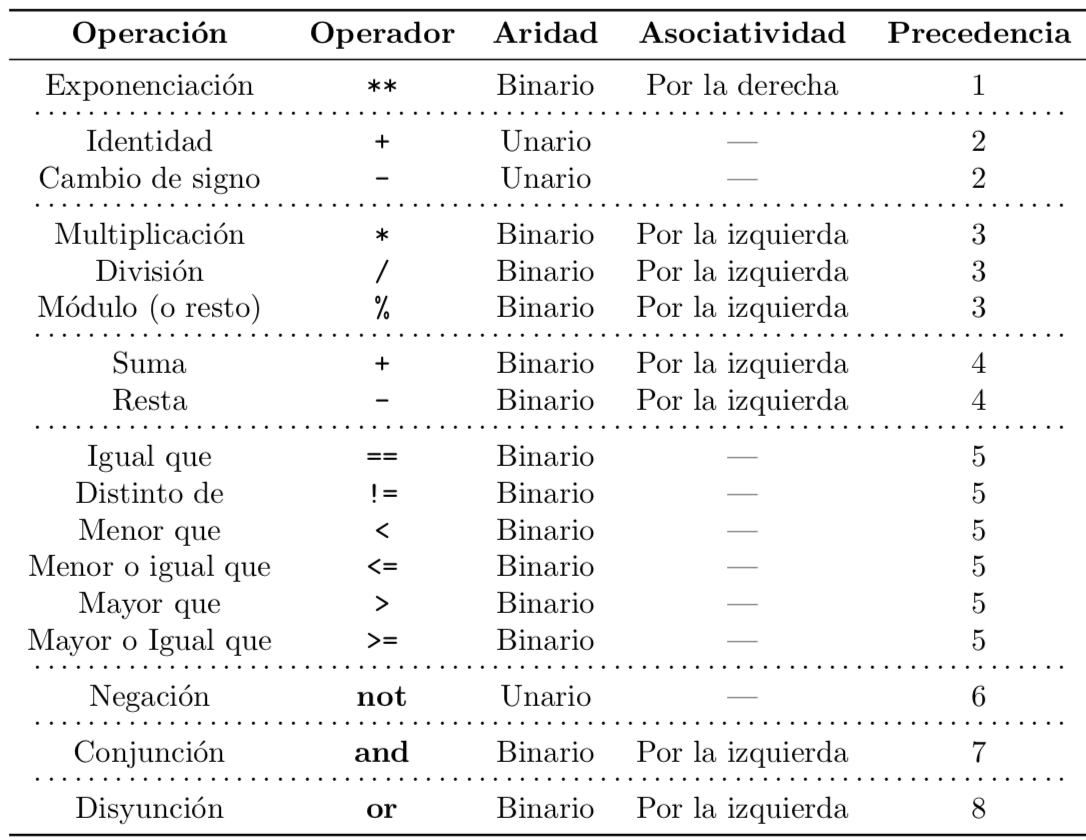
\includegraphics[width=.8\textwidth]{input/01-PythonLenguaje-fig/prioridadOperadores}}}

\caption{Orden de Precedencia \footnotesize Fuente: \texttt{Introducción a la Programación con Python} (página 37)}
\label{fig:precedencia}

\end{figure}


\paragraph{Mutabilidad y Casting.}

Una variables es \key{mutable} si se puede cambiar el valor de la variables sin cambiar su referencia en memoria.

La instrucción \pyv{id(var)} muestra la referencia de la variable {\tt var}.
Esta instrucción nos permite comprobar la mutabilidad de una variable.
Si se hacen dos asignaciones a una variable e \pyv{id()} cambia, la variables es inmutable.
Números, booleanos y strings son inmutables.  \hfill Compruébalo !!

	
	
El \key{casting} es el proceso por el que el valor de una variable se interpreta como otro tipo de dato.
Python no admite casting, pero sí tiene funciones para el \key{cambio de tipo}: 
	\pyv{int()}, \pyv{float()}, \pyv{str()}.




%%%%%%%%%%%%%%%%%%%%%%%%%%%%%%%%%%
%%%%%%%%%%%%%%%%%%%%%%%%%%%%%%%%%%

%%%%%%%%%%%%%%%%%%%%%%%%%%%%%%%%%%
%%%%%%%%%%%%%%%%%%%%%%%%%%%%%%%%%%
% --------------------------------------------------------
\label{subsec:ProgramacionEstructurada}

\subsection*{2.E.4 Programación Estructurada}
\addcontentsline{toc}{subsection}{2.E.4 Programación Estructurada}


La programación estructurada es un paradigma de programación que se basa en el \concepto{Teorema del Programa Estructurado}, propuesto por Böhm-Jacopini,  que demuestra que todo programa puede escribirse utilizando tres estructuras básicas, llamadas \key[red]{estructuras de control}:
\begin{itemize}
\item \key{Estructura secuencia}, consta de una secuencia de instrucciones directas.
\item \key{Estructura condicional}, que consta de una sentencias condicional y sus correspondiente cuerpos.
\item \key{Estructura iterativa}, que consta de bucles (o sentencias iterativas).
\end{itemize}


%--------------------------------------------------------------------------------
\paragraph{Estructura Secuencial.}

Consta de una secuencia de \key{órdenes directas}.
El conjunto de instrucciones \textbf{vienen dadas por el lenguaje} de programación.

\begin{itemize}
\item \key{Sentencias de Asignación}, consistentes en el paso de valores de una expresión o literal a una zona de la memoria.

\item \key{Lectura}, \pyv{input()}, consistente en recibir desde un dispositivo de entrada algún dato.

\item \key{Escritura}, \pyv{print()}, consiste en mandar a un dispositivo de salida algún valor.

\item \key{Tamaño}, \pyv{len()}, calcula el número de datos que tiene una secuencia (p.e. un string).

\item \key{Identificación}, \pyv{id()}, retorna la referencia de una variable.

\item \key{Tipo}, \pyv{type()}, indica el tipo de dato de un literal o de una variable.

\item ...
\end{itemize}

En \key[red]{Python} tenemos: 
	\begin{itemize}
	\item \textbf{Sentencias de asignación:} {\footnotesize \url{https://docs.python.org/3/reference/simple_stmts.html}}
	\item \textbf{Built-in Functions:} \footnotesize \url{https://docs.python.org/3/library/functions.html}
	\end{itemize}



%--------------------------------------------------------------------------------
\paragraph{Estructura condicional.}

Es  aquella que ejecuta ciertas órdenes si se cumple una condición booleana.

En \key[red]{Python} se usa la sentencia compuesta con cláusulas \cm{if}, \cm{elif}, \cm{else}.

\begin{itemize}
\item Condicional simple. 


\hfil
\begin{minipage}{.3\textwidth}
\begin{pyverbatim}[][frame=single, fontsize=\footnotesize]
if condicion:
    estructura
\end{pyverbatim}
\end{minipage} 
\begin{minipage}{.3\textwidth}
\begin{pyverbatim}[][frame=single, fontsize=\footnotesize]
if condicion: sentencia  # Inline
\end{pyverbatim}
\end{minipage}


\item Condicional doble. 


\hfil
\begin{minipage}{.3\textwidth}
\begin{pyverbatim}[][frame=single, fontsize=\footnotesize]
if condicion:
    estructura_if
else:
    estructura_else
\end{pyverbatim}
\end{minipage}
\begin{minipage}{.5\textwidth}
\begin{pyverbatim}[][frame=single, fontsize=\scriptsize]
var = exp_si_true  if  condicion else exp_si_false # Inline
\end{pyverbatim}
\end{minipage}



\item Condicional anidado.

\hfil
\begin{minipage}{.5\textwidth}
\begin{pyverbatim}[][frame=single, fontsize=\footnotesize]
if condicion1 [op condicion2 [op condicion3] ... ]:
    estructura_if
elif condicion:
    estructura_else_if
else  # Casi obligado si se usa elif.
    estructura_else
\end{pyverbatim}
\end{minipage}

\end{itemize}




%--------------------------------------------------------------------------------
\paragraph{Estructura Iterativa.}
%\small 


La versión imperativa de esta estructura consta de los siguientes pasos:

\begin{enumerate}\setlength{\itemsep}{0mm} \small
\item Se parte de una variable, que se llamará \key{variable de control} y que se inicializará a cierto valor. 

\item Entonces se comprueba una \key{condición} booleana donde interviene la variable de control. 

\item Si la condición es cierta, entonces se ejecutarán nuevas \key{estructuras}. 

\item Entres las \key{estructuras} habrá alguna secuencial que \key[magenta]{modifique la variable de control}.

\item Se vuelve paso 2.
\end{enumerate}

El proceso \key{se repite} hasta que la variable de control tome un valor que hace que la condición booleana es falsa.

En \cm[red]{Python} se usa la sentencia \cm{while}:

\begin{pyverbatim}[][frame=single, fontsize=\footnotesize]
control = valor_inicial
while expresion_booleana_con_la_var_de_control:
    estructuras
    modificar la variable de control
else: # opcional
   estructuras
\end{pyverbatim}


El bloque \cm{else} \key{no se realizará} si se ejecutara la sentencia \cm{break} en el bloque \cm{while}.


Existen dos sentencias, \cm{break} y \cm{continue}, que te pueden ser útiles:
%\small 

\begin{itemize}

\item \cm{break} 

\begin{itemize}
\item Solo puede ocurrir sintácticamente en un bucle \cm{for}\footnote{El bucle \cm{for} se estudiará en POO.} o \cm{while}.
\item Terminará el bucle adjunto más cercano y omitirá la cláusula opcional \cm{else}.
\end{itemize}

\item \cm{continue} 

\begin{itemize}
\item Solo puede ocurrir sintácticamente en un bucle \cm{for} o \cm{while}.
\item Continúa con la siguiente iteración del bucle  más cercano.
\item No ejecutará lo que aparezca después de \cm{continue} 
\end{itemize}

\end{itemize}


\begin{ejercicio}
Aquí hay un error muy común ?`cuál?

\hfil\begin{minipage}{.8\textwidth}
\begin{pyverbatim}[][frame=single]
control = 1
while control < 10:   # Se puede cambiar la condición
    if control % 2 == 0:
        continue
    elif control % 5 == 0:
        break
    print(control, end=" ")
    control = control + 1  # Se debe modificar la var. de control
else:
    print("No debería ejecutarse")
\end{pyverbatim}
\end{minipage}
\end{ejercicio}






%%%%%%%%%%%%%%%%%%%%%%%%%%%%%%%%%%
%%%%%%%%%%%%%%%%%%%%%%%%%%%%%%%%%%
% --------------------------------------------------------
\label{subsec:ProgramacionProcedimental}
\subsection*{2.E.5 Programación Procedimental}
\addcontentsline{toc}{subsection}{2.E.5 Programación Procedimental}

Una \key{función} es una \textbf{secuencia} de instrucciones identificada con un \textbf{nombre} que retorna un valor.  En \cm[red]{Python} una función puede retornar varios valores y, en este caso,
 \key{``empaqueta''} todos los datos de retorno en un tipo de datos llamado \key{tupla}. 


\hfil
\begin{minipage}{.65\textwidth}
{\footnotesize
\begin{pyverbatim}[][frame=single]
def nombre_funcion ( lista de parámetros ) -> tipo de dato de retorno:  
   estructuras de la función
   return valores 
\end{pyverbatim}
}
\end{minipage}



Un \key{procedimiento} es una función que no tiene la instrucción de retorno.

\hfil
\begin{minipage}{.65\textwidth}
{\footnotesize
\begin{pyverbatim}[][frame=single]
def nombre_procedimiento ( lista de parámetros ) [-> None]:  
   estructuras del procedimiento
\end{pyverbatim}
}
\end{minipage}


Si una función/método tiene $n$-parámetros podemos invocar a la función con $n$-argumentos de tal forma que el $1^{er}$ argumento se sustituya por el $1^{er}$ parámetro, el $2^{o}$ argumento por el $2^{o}$ parámetros, etc ... Son parámetros \key{posicionales}.


\begin{pyverbatim}[][frame=single]
def fun(a, b, c, d):  # Tiene 4 parámetros
    print(a, b, c, d)

fun(1, 2, 3, 4) # Invocamos con 4 parámetros posicionales.
\end{pyverbatim}


Los \key{k-últimos parámetros} de un función pueden ser \key{opcionales}.
	\begin{itemize}
	\item Los opcionales determinan un valor  \key[magenta]{literal} \key{ por defecto}. 
	\item \textbf{Primero} los obligatorios \textbf{y después} los opcionales (o por defecto).
	\end{itemize}

\begin{pyverbatim}[][frame=single]
def fun(a, b, c=3, d=4): #  2 posicionales + 2 opcionales.
    pass
\end{pyverbatim}


 \cm[red]{Python} permite invocar por \key{palabras claves} (keywords).
	\begin{itemize}
	\item Usar \textbf{keyword =}  especifica el nombre del parámetro en la invocación.
	\item El orden de los parámetros pueden cambiarse.
	\item En la declaración de la función, los keywords siempre se pondrán al final.
	\end{itemize}

\begin{pyverbatim}[][frame=single]
# Para la función anterior
fun(b=2, d=4, a=1, c=3) # Invocamos con 4 keywords.
fun(1, 2, d=4, c=3) # Los keywords al final
fun(d=4, 1, 2, c=3) # Incorrecto
\end{pyverbatim}



Cuando no se conoce el número de argumentos que se usarán, se usa el  \key{Packing Arguments} (empaquetamiento de argumentos) con el operador \key{*}.


\begin{pyconsole}[][frame=single]
def fun(*args):   # Empaquetará todos los argumentos
    print(args)

fun(1, 2, 3, 4)   # Invocación desempaquetada
\end{pyconsole}

En el ejemplo, todos los argumentos se agrupan en una \key{tupla}.

También existe el \key{Unpacking Arguments.} Dada una función/método con varios parámetros podemos empaquetar los argumentos con \key{*}.

\hfil
\begin{pyconsole}[][frame=single]
def fun(a, b, c, d):   # Desempaquetará si le envían \
    print(a, b, c, d)  # los argumentos empaquetados

lista = [1, 2, 3, 4] # Las listas las veremos más tarde.
fun(*lista)          # Invocación empaquetada
\end{pyconsole}



Para acceder a uno de lo argumentos empaquetados se usan \key{índices}:

\begin{pyconsole}[][frame=single, fontsize=\footnotesize]
def fun(*args): 
    print(len(args), args[1]) # Muestra el cardinal y el 2o argumento

fun(1, 2, 3, 4)
\end{pyconsole}


Estaría mejor acceder a ellos con un nombre (keyword). De hecho,
podemos \key{empaquetar y usar keywords} usando \textbf{diccionarios}, con \cm{**}. \textbf{Un diccionario es} como un array pero los índices se sustituyen por claves.

\begin{pyconsole}[][frame=single, fontsize=\footnotesize]
def fun(**kwargs): 
    print(f"{len(kwargs)} elementos", kwargs) # Muestra el diccionario

fun(a=1, b=2, c=3, d=4)    # Invocación con keywords
diccionario = {'p1': 1, 'p2': 2, 'p3':3}  # Los veremos
fun(**diccionario)         # Invocación con empaquetado
\end{pyconsole}




\noindent Si se quieren usar los 3 modos de pasar argumentos, el orden debe ser:
\begin{enumerate}
\item posicionales 
\item empaquetados sin keyword
\item empaquetados con keyword
\end{enumerate} 



\begin{pyconsole}[][frame=single, fontsize=\footnotesize]
def fun(a, b, *args, **kwargs): 
    print(a, b)  # Muestra los posicionales
    print(args)  # Muestra los empaquetados sin keyword
    print(kwargs)# Muestra los empaquetados con keyword

fun(1, 2, 3, 4, 5, p1=6, p2=7, p3=8)
\end{pyconsole}

\begin{ejercicio}
Se define \pyv{def func(x, y, op = "+")}. ?`Cuánto valdrá \cm{x}, \cm{y} y \cm{op} en los siguientes casos?

\begin{itemize*}
\item \pyv{func(2, 3, "*") }
\item \pyv{func( (2, 3), "*") }
\item \pyv{func( *(2, 3), "*")} \\
\item \pyv{func( *(2, 3, "*"))}
\item \pyv{func( (2, 3, "*"), 4)}
\item \pyv{func( *(2, 3, "*"), 4)}
\end{itemize*}
\end{ejercicio}



%--------------------------------------------------------------------------------
\paragraph{Docstrings.}

Toda función debe contener su \key{especificación informal}.
La documentación se hace en Python mediante \key{docstrings}: Cadenas que empiezan y terminan con triple comillas (simples o dobles)
Existen varios \key{formatos} (lenguajes de marcas):
\begin{itemize}
\item reStructuredText. El estandar de Python.
\item Google. La mejor alternativa "no-nativa".
\item Numpy. La propuesta de Numpy.
\item etc ...
\end{itemize}


\hfil\begin{minipage}{.4\textwidth}
\begin{pyverbatim}[][frame=single, fontsize=\footnotesize]
def func (x: int) -> str:
    """
    Función general que no hace nada
    reStructuredText
    
    :param x: La entrada, es entero
    :return: El valor de retorno
    """
    pass
\end{pyverbatim}
\end{minipage}
\begin{minipage}{.4\textwidth}
\begin{pyverbatim}[][frame=single, fontsize=\footnotesize]
def func (x: int) -> str:
    """
    Función general que no hace nada
    Google
    
    Args:
        x: La entrada, es entero

    Returns:
        El valor de retorno
    """
    pass
\end{pyverbatim}
\end{minipage}






%%%%%%%%%%%%%%%%%%%%%%%%%%%%%%s%%%%
%%%%%%%%%%%%%%%%%%%%%%%%%%%%%%%%%%
\paragraph{Funciones Lambda o Anónimas.}

El $\lambda$-cálculo es un sistema formal matemático desarrollado en los años 1930s diseñado para trabajar con la noción de  función, aplicación de funciones y  recursión. Proporciona una semántica simple para la computación y la primera simplificación es que el $\lambda$-cálculo \textbf{trata las funciones de forma anónima}.
La escritura anónima de $\color{red}{\displaystyle \operatorname {square\_sum} (x,y)=x^{2}+y^{2}}$ es  $\color{blue}{\displaystyle (x,y)\mapsto x^{2}+y^{2}}$.


En \key[red]{Python} las expresiones anónimas se llaman \key{Funciones Lambda} y
tiene la siguiente expresión: 

\centerline{\fbox{\pyv{lambda argumentos: expresión}}}

En la definición deberá tener en cuenta:
	\begin{itemize}
	\item Puede usar cualquier número de argumentos.
	\item Solo habrá una única expresión.
	\end{itemize}
	

\hfil\begin{minipage}{.4\textwidth}
\begin{pyconsole}[][frame=single, fontsize=\footnotesize]
el_doble = lambda x: x * 2
print(el_doble(10))
suma = lambda x, y: x + y
print(suma(4, 5))
acotado = lambda x: 4 <= x <= 8
print(acotado(5))
\end{pyconsole}
\end{minipage}


Son útiles junto con funciones clausura como \pyv{map()}, \pyv{filter()}, \cm{reduce}(), ... para trabajar con colecciones.  Se verán más adelante.






%%%%%%%%%%%%%%%%%%%%%%%%%%%%%%%%%%
%%%%%%%%%%%%%%%%%%%%%%%%%%%%%%%%%%

%--------------------------------------------------------------------------------
\subsection*{2.E.6 Programación Modular}
\addcontentsline{toc}{subsection}{2.E.6 Programación Modular}



Es un paradigma de programación que consiste en \key{dividir un gran programa} (posiblemente de  miles de líneas) \key{en módulos} (ficheros). 
Los módulos constan a su vez de \key{funciones}, \key{variables}, \key{clases}. 
Algunos módulos usarán otros módulos pero habrá uno (y solo uno), llamado \key{módulo principal}, que no puede ser usado por los demás módulos.
El módulo principal es el encargado de ir resolviendo cada una de las subtareas.


En \cm[red]{Python} la modularidad se consigue con \cm{import}. Ejemplo de uso de módulos:

\begin{minipage}{.31\textwidth}  
\begin{pyconsole}[][frame=single]
import math 
print("PI=", math.pi)
\end{pyconsole}
\end{minipage}
%
\begin{minipage}{.31\textwidth}
\begin{pyconsole}[][frame=single]
import math as m
print("PI=", m.pi)
\end{pyconsole}
\end{minipage}
%
\begin{minipage}{.33\textwidth}
\begin{pyconsole}[][frame=single]
from math import pi, cos
print("cos(PI)=", cos(pi))
\end{pyconsole}
\end{minipage}




%%%%%%%%%%%%%%%%%%%%%%%%%%%%%%%%%%
%%%%%%%%%%%%%%%%%%%%%%%%%%%%%%%%%%

%--------------------------------------------------------------------------------
\label{subsec:ClasesEnPython}
\subsection*{2.E.7 Programación Orientada a Objetos \label{subsec:POO}}
\addcontentsline{toc}{subsection}{2.E.7 Programación Orientada a Objetos}


La estructura básica para definir una clase en \cm[red]{Python} es la siguiente:

\hfil \begin{minipage}{.75\textwidth}
\begin{pyverbatim}[][frame=single]
class NombreDeLaClase: # Notación Camel
    def __init__(self, p1, p2, ...):
        self._var1 = p1
        self._var2 = p2
        ...  # más atributos
        
    def metodo1 (self, parametros):
        acciones
            
    def metodo2 (self, parametros):
        acciones
            
     .... # más métodos
        
objeto = NombreDeLaClase(argumentos para __init__)
\end{pyverbatim}
\end{minipage}

\

Todos los métodos que tienen la forma: \cm[blue]{\_\_metodo\_\_}{\tt (...)} se denominan    \key{métodos mágicos}. Destacamos:

\begin{itemize}

\item \pyv{__new__(cls, ...)}. Es el método creador.  \textbf{No debe escribirse nunca}.

\item \pyv{__init__(self, ...)}.   \textbf{Es un método inicializador} de instancia que se invoca siempre, una vez construido el objeto con \pyv{__new__(cls, ...)}.

\item etc ...
\end{itemize}


Trabajar con \key{TDAs} como modelos \key{ayuda} muchísimo  a la resolución de problemas y  diseño de algoritmos; pero al final hay que implementarlos en un lenguaje de programación usando sus \key{tipos de datos integrados}.  Todos los tipos de datos integrados en Python son objetos y, por tanto, si queremos construir nuevos tipos de datos debemos saber cómo construir y manipular nuevos objetos.

Deberá tener presente que Python es un lenguaje de POO puro. En consecuencia, cualquier operación que realice conlleva manipular los atributos del objeto y, por tanto, invocará de forma directa o indirecta a los métodos del objeto.

Por ejemplo, en \underline{todos} los \textbf{Tipos de Datos Numéricos} tenemos estos miembros/métodos y operaciones:
	\begin{itemize}
	\item Miembros: \cm[blue]{.real}, \cm[blue]{.imag}
	\item Métodos: \cm[blue]{.conjugate()}, 
	\item Operaciones: \cm{+}, \cm{-}, \cm{*}, \cm{/}, \cm{//}.
	\item Los métodos mágicos sobre operaciones matemáticas, asignaciones extendidas, operaciones unarias y operaciones de comparación.
	\end{itemize}

Esto quiere decir que cuando realice una operación numérica  invocará al método mágico correspondiente. Por ejemplo,  
	\begin{itemize}
	\item Cuando escriba \key{3+5}, internamente se ejecutará \pyv{3.__add__(5}). Siendo el \key{3} y el \key{5} dos objetos.
	\item Si escribe \key{3-5}, internamente se ejecutará \pyv{3.__sub__(5)}.
	\item etc ...
	\end{itemize}

Lo mismo ocurre cuando invoque a un función sobre un número. Por ejemplo, invocando a \key{abs(3}) estará invocando a \pyv{3.__abs__()}.  También ocurre lo mismo al usar operadores de comparación: usar \cm{<} es invocar al método \pyv{.__lt__()}, usar \cm{==} invocará al método \pyv{.__eq__()}, etc ...

De entre todos los operadores el más esencial es sin duda la asignación \cm{=}. Cada vez que realice una asignación de la forma estará construyendo un objeto nuevo y cada vez que se crea un objeto nuevo se invocará al método \pyv{.__init__()}. Esto es muy importante a tener en cuenta porque:

\begin{itemize}
\item A ser un lenguaje no tipado, la asignación determina su tipo. En consecuencia una variable puede referenciar incialmente a un entero para terminar referenciando a una lista.

\begin{pyverbatim}[][frame=single]
a = 2  % a es un objeto entero
a = 2 == 3  % a es un objeto booleano
a = NombreDeLaClase(p1, p2) % a es un objeto de NombreDeLaClase
\end{pyverbatim}

 
 
\item Todas las variables tienen un ámbito local salvo que  se diga lo contrario (se explicará  posteriormente).
\end{itemize}

\noindent Para completar los \textbf{Tipos de Datos Numéricos} en  Python, indicar que se tienen los siguientes.

\begin{itemize}	
\item \textbf{Enteros:}
	\begin{itemize}
	\item Una variable se declara entera si se le asigna un número sin punto decimal.
	\item Función constructora: \cm{int()}. 
	\item Métodos: \cm[blue]{.bit\_length()}: N$^o$ de bits necesarios.
	\item Funciones: \key{bin}(n). Convierte a binario.
	\end{itemize}
	
\item \textbf{Reales:}
	\begin{itemize}
	\item Una variable se declara real si se le asigna un número con punto decimal.
	\item Función constructora: \cm{float()}. 
	\item Métodos: \cm[blue]{.is\_integer()}: True si el valor es igual al de su parte entera.
	\end{itemize}
	
\item \textbf{Complejos:}
	\begin{itemize}
	\item Constructor: \cm{complex([real[, imag]])}
	\end{itemize}
\end{itemize}

Podemos aumentar el conjunto de datos numéricos usando librerías.
Destacamos aquí el módulo \textbf{Fracciones:}
	\begin{itemize}
	\item Requiere \cm{from fractions import Fraction}
	\item Constructores: \cm{Fraction(numerator=0, denominator=1)}, \cm{Fraction(float)}, \cm{Fraction(string)}, ...
	\item Miembros: \cm[blue]{.numerator}, \cm[blue]{.denominator}
	\item Métodos: \cm[blue]{.as\_integer\_ratio()}: simplifica la fracción.
	\item \url{https://docs.python.org/3/library/fractions.html}
	\end{itemize}	
	
\


Otros tipos de datos integrados son los \textbf{Tipos de Datos Booleanos.}
Usa las constantes True y False. Una variable a la que se le asigne uno de estos valores será una variable booleana.  Las expresiones booleanas se construyen con:
	\begin{itemize}
	\item Comparaciones: \cm{x == y}, \cm{x != y}, \cm{x > y}, \cm{x >= y}, \cm{x <\ y}, \cm{x <= y}
	\item Operaciones: \cm{e1 and e2}, \cm{e1 or e2}, \cm{not e}
	\end{itemize}
	
Recuerde que todas estas operaciones invocará a sus correspondiente método mágicos.
	

Los TDAs más relevantes requieren el uso de colecciones.
\cm[red]{Python} proporciona un conjunto de tipos de datos llamados \textbf{secuencias} (colecciones) o tipos de datos secuenciales. Se explicarán con más detenimiento en sesiones posteriores (de teoría/prácticas).



\paragraph{Recuerde seguir  PEP 8 para las normas de estilo.}
\paragraph{PEP 8 -- Style Guide for Python Code: \url{https://www.python.org/dev/peps/pep-0008/}
}	








